\chapter{模型介绍}
\label{chapter:model}
\section{指数平滑模型(Holt)}
Holt 线性趋势方法,也称为 Holt 双参数指数平滑法,是一种时间序列预测技术,用于处理显示出明显线性趋势的数据。Holt 线性趋势方法包含两个方程:一个是水平方程,另一个是趋势方程。

1. 水平方程计算当前时间点的平滑水平值:
\begin{equation}
\ell_t = \alpha y_t + (1 - \alpha)(\ell_{t-1} + b_{t-1}) 
\end{equation}

2. 趋势方程计算当前时间点的趋势值:
\begin{equation}
b_t = \beta(\ell_t - \ell_{t-1}) + (1 - \beta)b_{t-1} 
\end{equation}

其中:$\ell_t$  是在时间  t  的水平成分。$\alpha $ 是水平平滑参数, $0 < \alpha < 1 $。$y_t$  是在时间  t  的实际观测值。$b_{t-1} $ 是在时间 $ t-1 $ 的趋势成分。$b_t $ 是在时间  t  的趋势成分。
$\beta $ 是趋势平滑参数,$ 0 < \beta < 1 $。

最终的预测方程结合了水平和趋势成分来生成对未来时间点的预测:
\begin{equation}
\hat{y}_{t+h|t} = \ell_t + hb_t 
\end{equation}
这里,$ \hat{y}_{t+h|t}$  是在时间  t  基础上对  h  期后的预测值。

Holt 线性趋势方法特别适用于那些具有线性趋势、数据量较少但无季节性的时间序列。通过选择适当的 $ \alpha$和  $\beta$  值,可以调整模型对水平和趋势的敏感程度,进而影响预测的准确度。
在本报告中,将2014、2016、2018年的城乡互联网使用程度的数据通过指数平滑法进行2020和2022的预测。

\section{LSTM}
LSTM从被设计之初就被用于解决一般递归神经网络中普遍存在的长期依赖问题,使用LSTM可以有效的传递和表达长时间序列中的信息并且不会导致长时间前的有用信息被忽略(遗忘)。

一个LSTM单元主要由以下几个部分组成:遗忘门、输入门、细胞更新和输出门。简化图如下:

\begin{figure}
    \centering
    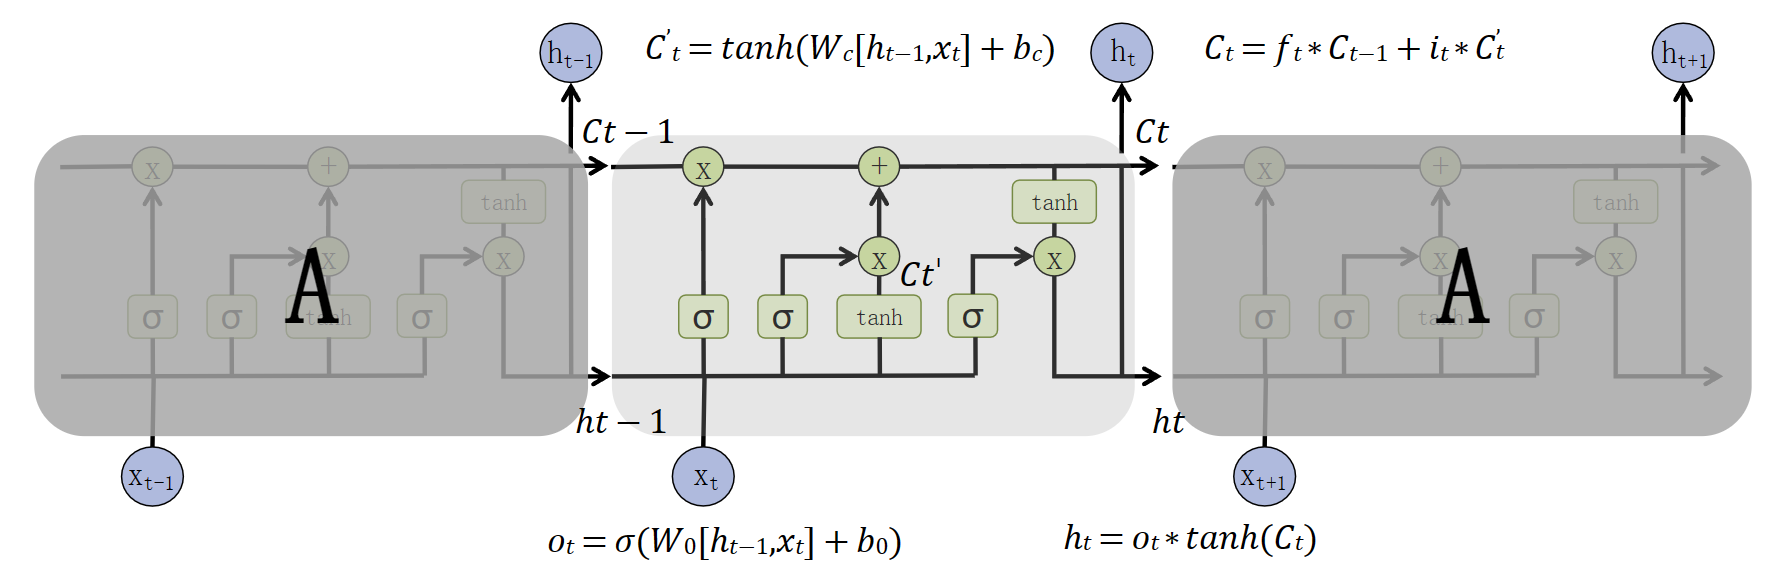
\includegraphics[width=0.9\linewidth]{figures/30.png}
    \caption{LSTM原理图}
    \label{fig:enter-label}
\end{figure}

假设在时间步 t,LSTM接收到输入向量 $x_t$ 和上一个时间步的输出 $h_{t-1}$以及细胞状态 $c_{t-1}$。

1. 
遗忘门:
\begin{equation}
f_t = \sigma(W_f \cdot [h_{t-1}, x_t] + b_f)
\end{equation}

$f_t$ 是遗忘门的输出,$W_f$ 是遗忘门的权重矩阵,$b_f$ 是偏置项,$\sigma$ 是$sigmoid$函数,它确保输出值在0和1之间,决定了要从细胞状态中遗忘多少信息。

2. 
输入门和候选细胞状态:
\begin{equation}
i_t = \sigma(W_i \cdot [h_{t-1}, x_t] + b_i)
\\
\tilde{c}_t = \tanh(W_c \cdot [h_{t-1}, x_t] + b_c)
\end{equation}

输入门决定了我们将在细胞状态中更新多少新信息,而候选细胞状态则提供了一个新的候选信息集,这些信息可能会被添加到细胞状态中。

3. 
细胞状态更新:
\begin{equation}
c_t = f_t * c_{t-1} + i_t * \tilde{c}_t
\end{equation}


当前细胞状态$c_t$是前一状态$c_{t-1}$经过遗忘门“遗忘”一部分后,与新的候选细胞状态经过输入门“筛选”一部分后相加得到的。

4. 
输出门和输出值: 
\begin{equation}
o_t = \sigma(W_o \cdot [h_{t-1}, x_t] + b_o)
\\
h_t = o_t * \tanh(c_t)
\end{equation}

输出门决定了哪些细胞状态的信息将输出,而输出值$h_t$则是这部分信息经过处理后用于传递到下一个LSTM单元或用于当前单元的输出。

这些公式共同定义了LSTM单元如何通过时间传递和更新信息,使其能够捕捉长期依赖关系。在本篇报告中,在预测数字农业渗透率、城乡就业人员、城乡总人口时采用了LSTM对接下来几年进行了时间预测。

\section{DLF}
双逻辑函数(Double Logistic Function, DLF)是一种适用于受到多重因素影响,既有增长又有减少的进行动态复杂变化的数学模型,比如人口。双逻辑函数通过结合两个逻辑函数,更加灵活地模拟出人口先增长后减少或反之的变化情况,如下图所示:
\begin{figure}[h]
    \centering
    \begin{minipage}[b]{0.45\textwidth}
        \centering
        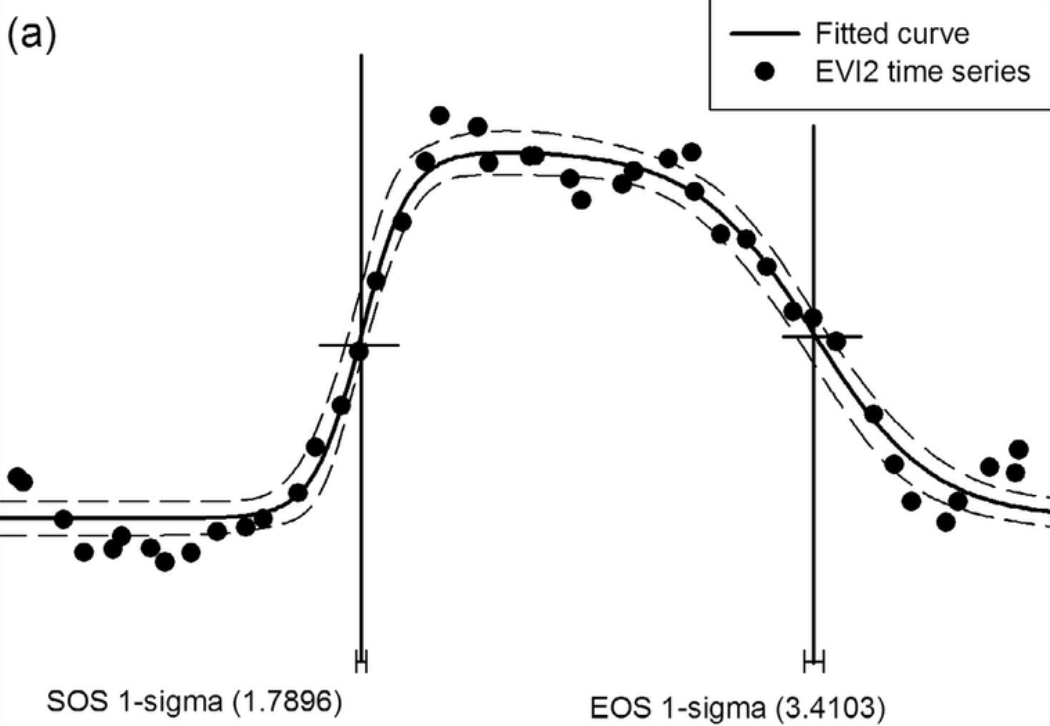
\includegraphics[width=\linewidth]{figures/53.png}
  
        \label{fig:first-image}
    \end{minipage}
    \hspace{0.05\textwidth} % Optional, add space between the images
    \begin{minipage}[b]{0.45\textwidth}
        \centering
        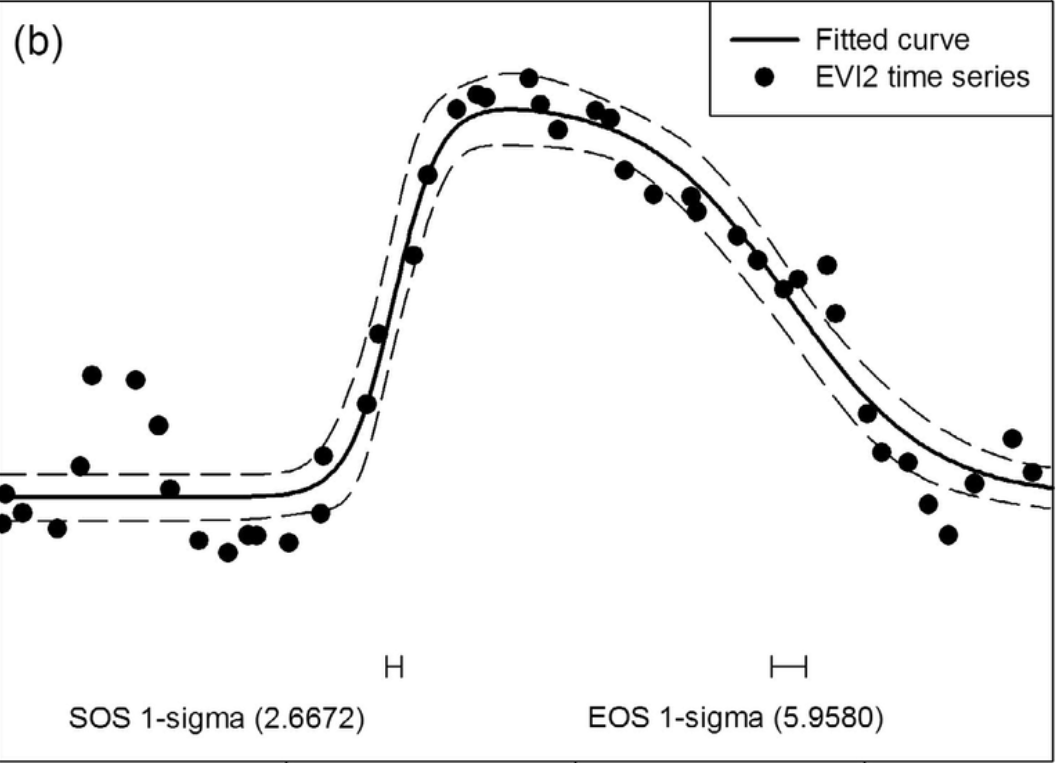
\includegraphics[width=\linewidth]{figures/54.png}
        
        \label{fig:second-image}
    \end{minipage}
    \caption{双逻辑函数进行曲线拟合}
\end{figure}

双逻辑函数的模型公式为:

\begin{equation}
P(t) = \frac{K}{1 + e^{-r(t - t_0)}} + \frac{L}{1 + e^{-s(t - t_1)}}
\end{equation}

其中$K$和$L$表示增长和减少的幅度,$r$和$s$是相应的增长率,$t_0$和$t_1$是拐点时间。

相比单一逻辑函数,双逻辑函数具有灵活性强、精度高和直观性好的优势。假设一个城市在某段时间内经历了快速人口增长,随后由于某些原因(如经济衰退、自然灾害)导致人口减少。利用双逻辑函数,可以分别设定增长和减少的幅度、速度和时间点,精确模拟出这一变化过程,提供有效的预测和分析工具。

\section{DLF-LSTM}
由于我们所获得的数据大部分与年份相关,且数据量较少,容易产生过拟合的情况。单纯依赖数学模型难以准确捕捉数据中的依赖关系,也无法拟合随着外部因素动态变化的信息。因此,我们考虑将两种模型进行融合,结合数学模型的精确性和机器学习模型的适应性,以提高整体模型的表现。

在本文中,我们选择双逻辑函数(DLF)和长短期记忆网络(LSTM)作为基学习器,同时处理相同的训练集,将得到的参数放入同一个数据集,并作为输入值输入到元学习器中。

\begin{figure}[H]
    \centering
    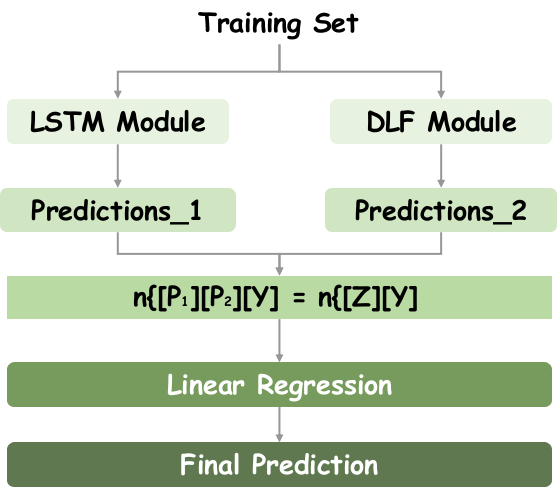
\includegraphics[width=0.45\linewidth]{figures/51.png}
    \caption{DLF-LSTM模型架构图}
    \label{fig:enter-label}
\end{figure}

尽管线性回归在处理非线性数据时可能存在一定的局限性,因为它本质上是线性的,但由于我们已经使用了双逻辑函数和LSTM对数据进行了非线性处理,线性回归可以有效地作为元学习器来整合这些非线性模型的输出结果。
\begin{algorithm}[H] % This keeps the algorithm where it is in the text
\caption{DLF-LSTM}
\begin{algorithmic}[1]
\State Initialize models: Double Logistic Function (DLF) and LSTM
\State Prepare dataset $D$, split into $D_{\text{train}}$ and $D_{\text{test}}$
\State \textbf{Train DLF and LSTM:}
\For{$(x_i, y_i) \in D_{\text{train}}$}
    \State Predict $y_{\text{DLF}}^i \leftarrow \text{DLF}(x_i)$ and $y_{\text{LSTM}}^i \leftarrow \text{LSTM}(x_i)$
    \State Store predictions
\EndFor
\State Combine predictions into new feature set $X_{\text{meta}}$
\State \textbf{Train Linear Regression Meta-Learner:}
\State Train on $X_{\text{meta}}$ to predict $y_i$
\State \textbf{Evaluate Model on $D_{\text{test}}$:}
\For{$(x_i, y_i) \in D_{\text{test}}$}
    \State Predict $y_{\text{pred}}^i$ and compute accuracy
\EndFor
\State Output the overall performance
\end{algorithmic}
\end{algorithm}
使用“堆叠回归”(Stacked Regression)的方法将DLF和LSTM融合,能够在一定程度上实现两者的互补,充分发挥各自的优势,从而提高整体模型的预测准确性和鲁棒性。

\section{模型对比}
我们对融合之后的 DLF-LSTM 模型与其他模型及融合之前的模型进行了对比,比较了不同机器学习模型在测试集上的性能,尤其是在误差(MSE、RMSE)和模型解释能力(R²)方面,结果如下图所示。

\begin{figure}[H]
    \centering
    \begin{subfigure}[b]{0.6\linewidth}
        \centering
        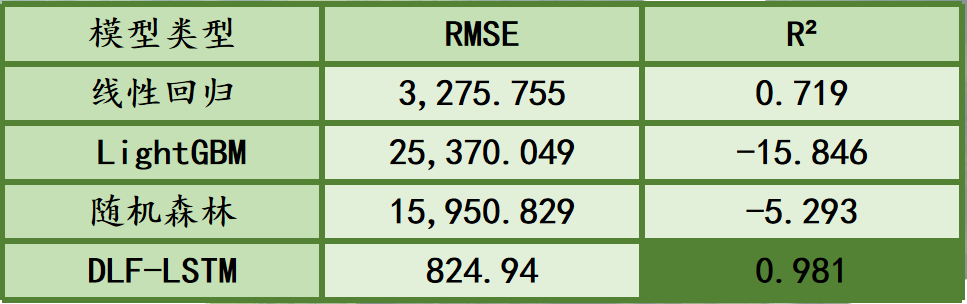
\includegraphics[width=\linewidth]{figures/55.png}
     
        \label{fig:enter-label-1}
    \end{subfigure}%
    \\
    \begin{subfigure}[b]{0.6\linewidth}
        \centering
        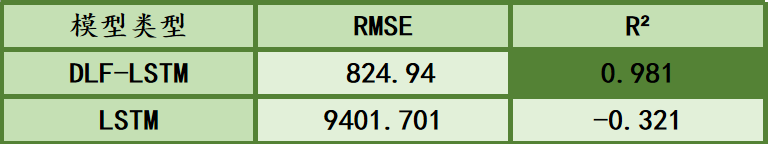
\includegraphics[width=\linewidth]{figures/56.png}
        
        \label{fig:enter-label-2}
    \end{subfigure}
    \caption{与原先模型的对比}
    \label{fig:combined-label}
\end{figure}

从图表中可以看出,DLF-LSTM 模型在所有指标上表现最优,具有最低的 MSE 和 RMSE,以及非常高的 R² 值,显示了出色的预测能力和数据拟合度。相比之下,其他模型的表现则不尽如人意。例如,随机森林模型出现了过拟合现象;LightGBM 的 R² 值甚至为负,显示其在测试集上的表现非常差;线性回归模型的准确率不高,难以胜任复杂的预测任务。

对比融合之前的模型,LSTM 的 RMSE 明显高于 DLF-LSTM,表明其在测试集上的预测误差较大。此外,LSTM 的 R² 值为负,表示其在测试集上的表现甚至比基于数据平均值的简单模型还要差,这是典型的过拟合迹象。

总体而言,DLF-LSTM 模型展示了非常低的误差和高度的数据拟合能力(R² 接近 1),表明其具有优越的性能,能够有效地避免过拟合,并在未见数据上提供可靠的预测。而标准 LSTM 模型则可能需要进一步的参数调整和正则化以改善其泛化能力。

这个对比结果表明,DLF-LSTM 模型在各种指标上均表现出色,是一个更为优越的特定于少量时序数据的选择,能够在复杂的预测任务中提供更高的准确性和可靠性。
